\documentclass[11pt]{article}

\usepackage{amsmath}
\usepackage{setspace}
\usepackage{amssymb}
\usepackage{changepage}
\usepackage{graphicx}
\usepackage[a4paper, margin=0.5in]{geometry}

\DeclareMathOperator*{\argmin}{arg\,min}

\setstretch{1.3}

\hbadness=10000
\setlength{\parindent}{0pt}

\newcommand\numberthis{\addtocounter{equation}{1}\tag{\theequation}}

\begin{document}
    \begin{center}
        \Large \textbf{STAT3006 Worksheet 05}
    \end{center}

    \Large \textbf{1. Random Forest: Splitting Bias and Feature Subsampling}

    \large Consider a random forest regression estimator 

    \begin{align*}
        f_{RF}(\mathbf{x}) = \frac{1}{B}\sum_{b = 1}^B f^{(b)}(\mathbf{x})
    \end{align*}

    where each tree is grown fully and uses feature subsampling of size $q$ at each split.

    \begin{adjustwidth}{1em}{1em}
        (a) Consider a feature $\mathbf{x}_j$ that is weakly predictive but correlated with a strong
        feature $\mathbf{x}_k$. Explain why bagging tends to underuse $\mathbf{x}_j$ \\ 

        \textbf{Answer:} The bagging algorithm works by generating $B$ subsamples of the training
        data by picking random datapoints with replacement. It then fits $B$ trees for each
        subsample. \\ 

        Since $\mathbf{x}_k$ is a strong feature, we can expect most, if not all $B$ trees to
        choose $\mathbf{x}_k$ at the first split, in which the CART algorithm might reach its
        stopping condition before it ends up choosing the weakly predictive feature $\mathbf{x}_j$.
        In other words, it underuses $\mathbf{x}_j$ \\ 

        (b) Run the attached Jupyter Notebook titled "WS.ipynb" which simulates the above situation
        and confirm your observations \\

        \textbf{Answer:} Consider the following code snippet and output \\

        \begin{center}
            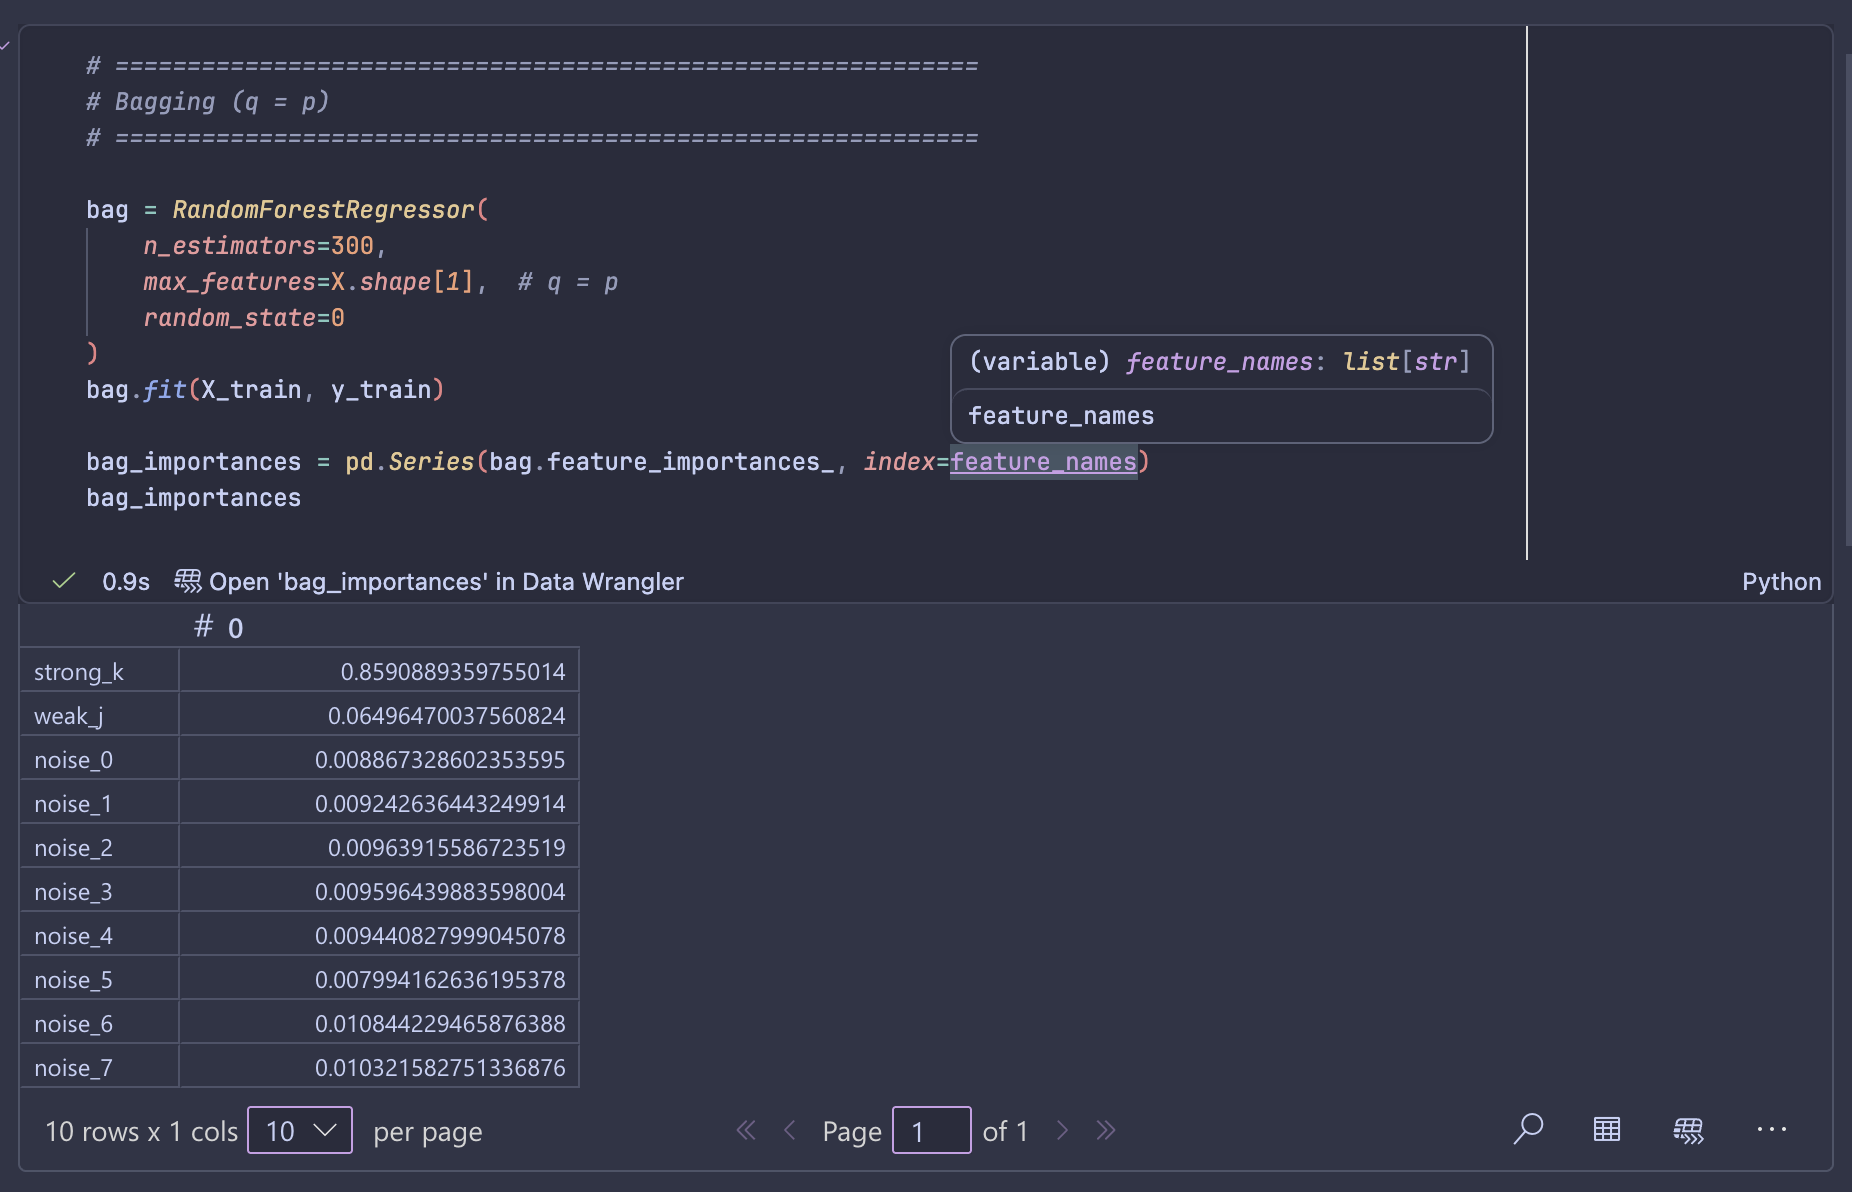
\includegraphics[width=0.8\textwidth]{w5q2.png}
        \end{center}

        Here we can see that a most of the feature importance is placed in the strong predictor
        $\mathbf{x}_k$ in the bagging algorithm, confirming our observations from part (a). \\ 

        (c) Explain how feature subsampling in random forests mitigates the issue in part (a) \\ 
        
        \textbf{Answer:} In the Random Forest algorithm, it works similarly to bagging where $B$
        subsamples of the training data are generated at random with replacement. However for each
        tree, we also pick a subset of the original features of length $q, q \leq p$ that we use to
        train the tree. \\ 

        This mitigates the issue found in part (a) as in some trees, the feature subset may exclude
        the strong feature but include the weak predictor. We confirm our observation by running the
        below code snippet: \\ 

        \begin{center}
            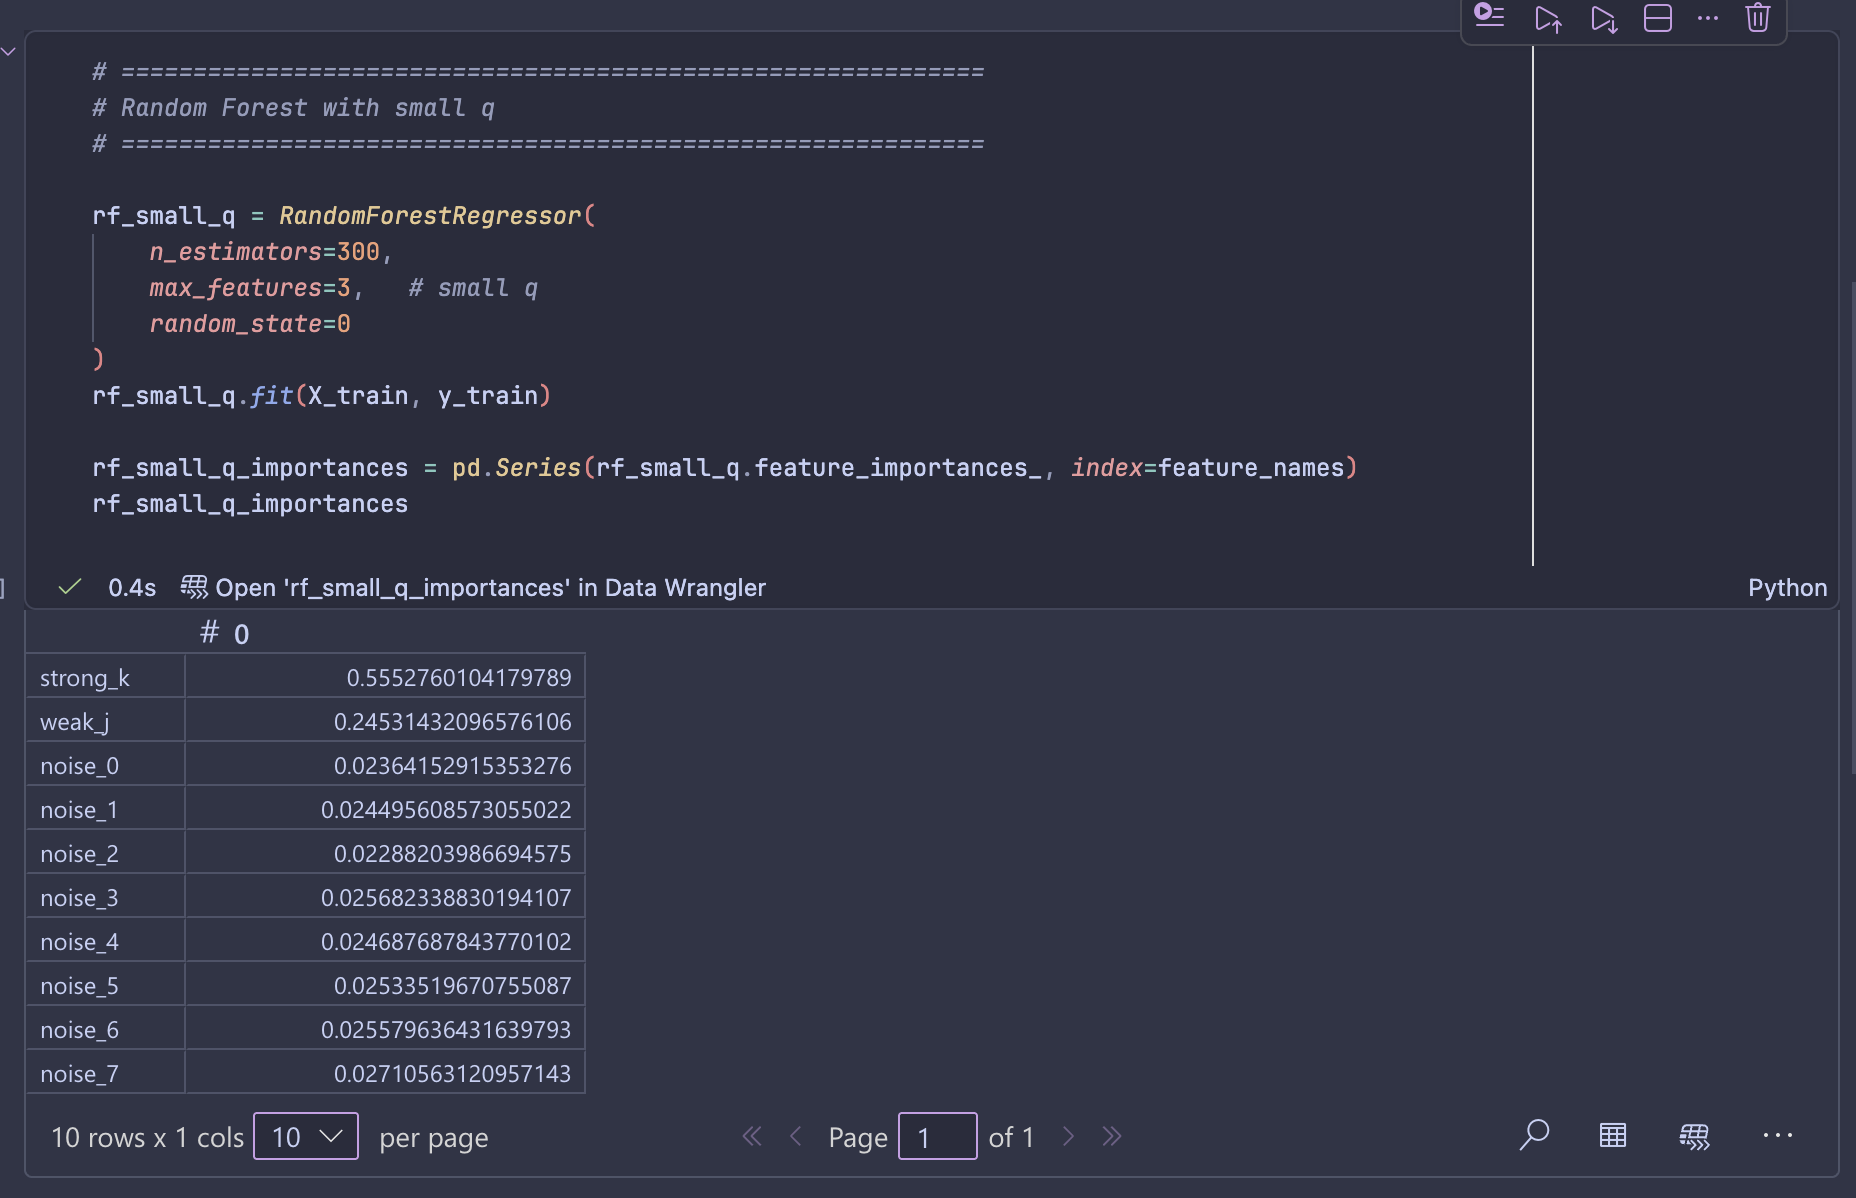
\includegraphics[width=0.8\textwidth]{w5q3.png}
        \end{center}

        (d) Suppose $q$ is extremely small (e.g. $q = 1$). Discuss the bias-variance trade-off in
        this extreme regime. \\ 
        
        \textbf{Answer:} Since every tree has only one feature, there is no greedy behaviour where
        the CART algorithm picks the best feature to determine the best split, it just chooses the
        single feature that it is given. Since that single feature is chosen at random, the splits
        are essentially random and therefore the trees will have low correlation. Recall the
        variance of an ensemble, 

        \begin{align*}
            \frac{1 - \rho}{B}\sigma^2 + \rho \sigma^2
        \end{align*}

        Since $\rho \approx 0$, as $B\to\infty$ we decrease the overall variance of the ensemble
        down to zero. On the other hand, since each tree uses its given feature at the split point
        it will train the tree on just that one feature. In other words, each tree in the ensemble
        has high bias, and since the bias of the ensemble is just the average of the bias of it's
        trees, since all trees have high bias then the ensemble will also have high bias. \\ 

        (e) Run the attached Jupyter Notebook titled "q.ipynb", which studies the effect of $q$ on
        bias, variance, and predictive performance under two different data-generating regimes

        \begin{itemize}
            \item Regime A: (Sparse Strong Signal)

                \begin{align*}
                    f_A(x) = \sin(x_0) + 0.5x_1
                \end{align*}

            Where only two features carry signal and the remaining $p - 2$ features are pure noise
        \item Regime B: (Dense Weak Signal)
            
                \begin{align*}
                    f_B(x) = \frac{1}{10}\sum_{j = 0}^9 \sin(x_j)
                \end{align*}

            Where ten features contribute weakly and the remaining $p - 10$ features are noise. 
        \end{itemize}

        Explain your observations \\ 

        \textbf{Answer:} Consider the following results: \\ 

        \begin{center}
            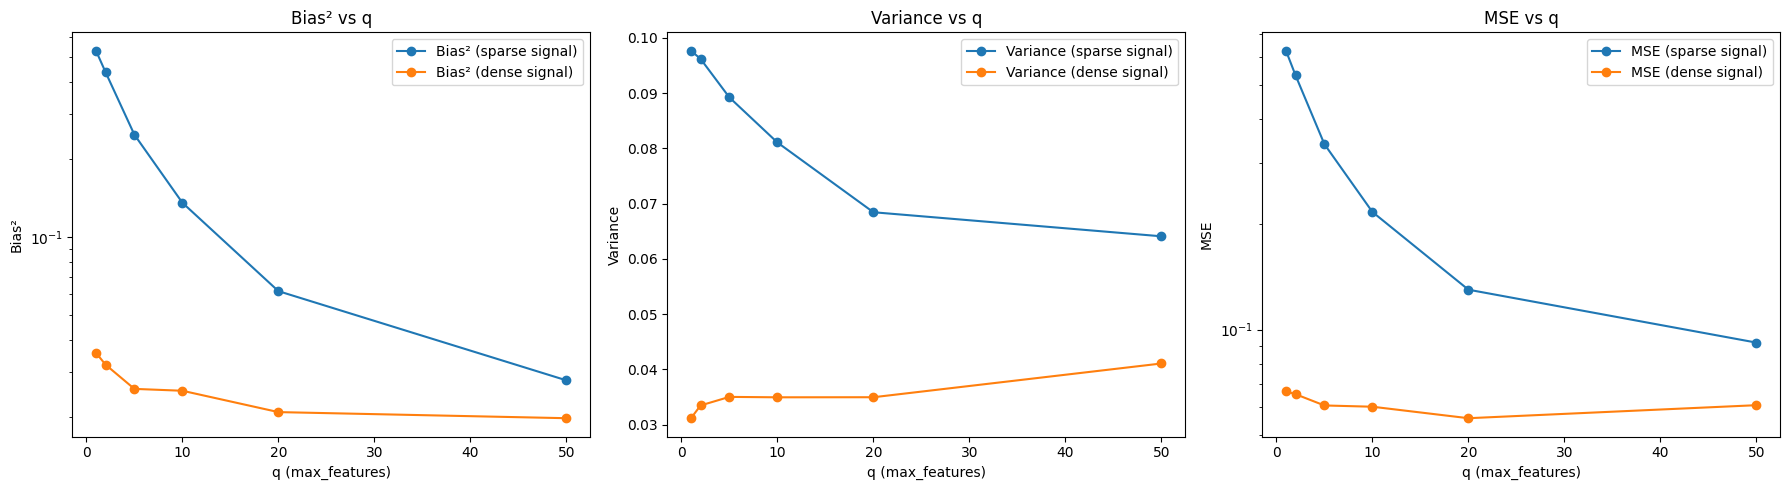
\includegraphics[width=0.9\textwidth]{w5q5.png}
        \end{center}

        \textbf{Bias:} For smaller values of $q$, the random forest algorithm can only choose from
        the subset of $p$ features to split, which leads to high bias for each individual trees.
        This leads to high bias for the whole ensemble. As $q$ grows, each tree becomes more
        flexible and therefore bias decreases. \\ 

        \textbf{Variance:} For smaller $q$, the sparse signal ensemble results in high variance as
        for a significant number of trees, it will most likely pick the noisy features ($p - 2$). As
        $q$ grows, there is a higher chance that the two strong features are picked in which the
        CART algorithm will pick these to split on, therefore reducing variance as the tree captures
        the behaviour of the data generating distribution. \\ 

        On the other hand, we can see that the dense singal starts at low variance for small $q$. As
        explained in the previous question, this results in low variance as $\rho \approx 0$,
        therefore the variance of the ensemble can be determined via

        \begin{align*}
            \frac{1}{B}\sigma^2
        \end{align*}

        However as $q$ grows, $\rho$ increases and leads to higher variance. Another explanation is
        that since the 10 features used contribute weakly, adding other noisy features to the
        training algorithm will make the tree learn the noise as opposed to the true data-generating
        distribution, leading to higher variance. \\ 

        \textbf{MSE:} MSE is formulated by

        \begin{align*}
            \text{MSE} = \text{Variance} + \text{Bias}^2
        \end{align*}

        Using this equation, we can trivially reason about why the MSE behaves as seen above by
        looking at how the variance and bias squared behaves for each data generating distribution.
        \\ 

        (f) Now explore the role of te number of trees $B$ in terms of bias, variance and prediction
        performance. Run the Jupyter Notebook titled "B.ipynb", which fits random forests with
        varying $B$ to both regression functions above. What do you observe? Explain your findings.
        \\ 

        \textbf{Answer:} Consider the following outputs: \\

        \begin{center}
            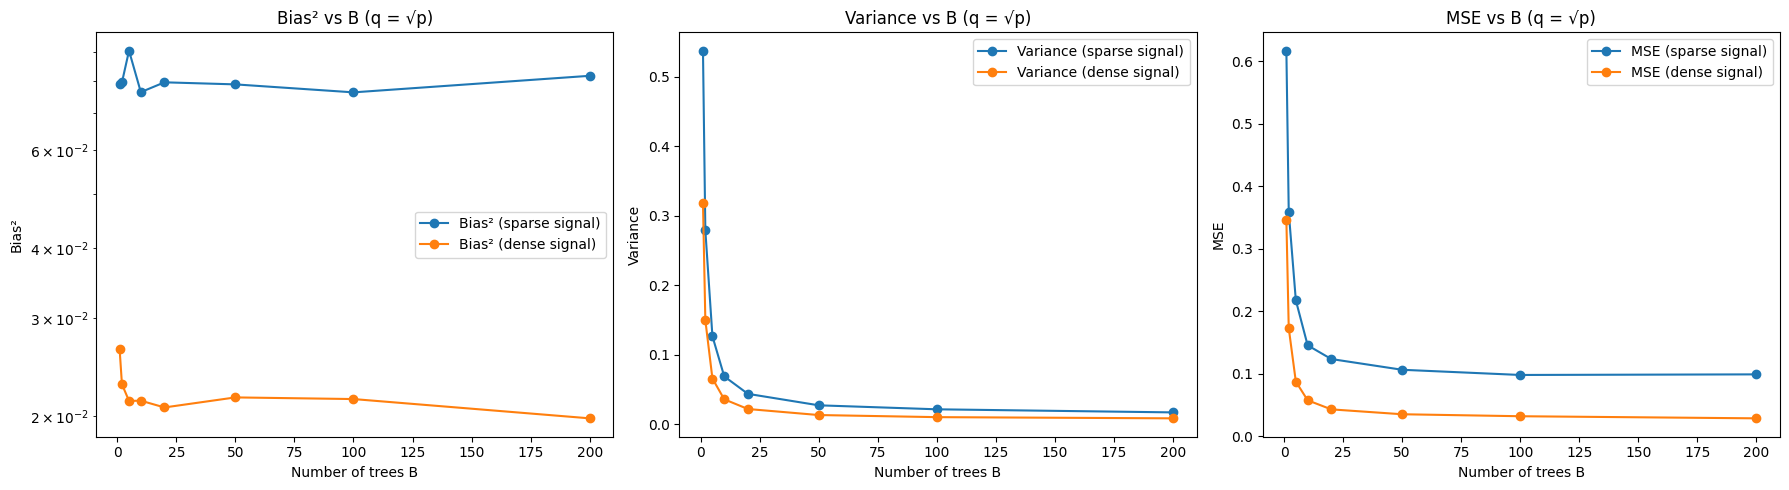
\includegraphics[width=0.9\textwidth]{w5q6.png}
        \end{center}

        \textbf{Bias:} We can see here that for both data-generating distributions, bias stays about
        the same for all values of $B$, this is because bias is heavily dependent on the size of the
        feature subset $q$ which in this experiment is a constant value. \\ 

        \textbf{Variance:} Again recall the equation for the variance of an ensemble

        \begin{align*}
            \frac{1 - \rho}{B}\sigma^2 + \rho \sigma^2
        \end{align*}

        As $B$ increases, the first term approaches zero in which the variance of the ensemble
        mostly dependends on the second term. \\ 

        \textbf{MSE:} Again we can trivially reason about the behaviour of the MSE by looking at the
        variance and bias.
    \end{adjustwidth}


\end{document}
